%-------------------------------------------------------------------------------------------------------
%-------------------------------------------------------------------------------------------------------
%-------------------------------------------------------------------------------------------------------
\subsection{Structure of section}
Every section of this chapter is a simulation of the future application. Every simulation is has his own scene (Showed in this document with some images, for example as in Figure: \ref{fig:VREP_scene_example}). This scenes contains the requited quadrotors and targets in order to test the behavior previous real results. Results of vision algorithm is showed in the vrep console(Figure: \ref{fig:Ground_Tracking_VREP_Console}). \\

\begin{figure}[h]
	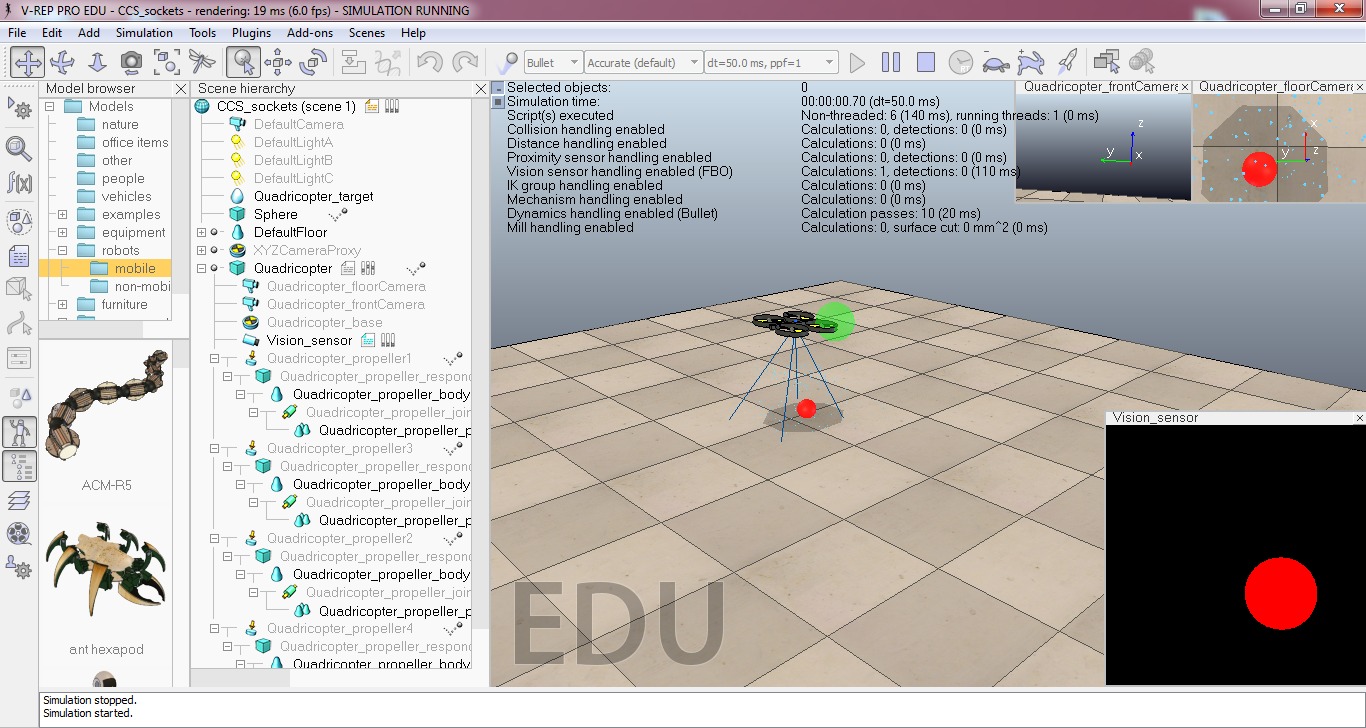
\includegraphics[width=0.7\textwidth,natwidth=1366,natheight=728]{../Images/c3/ground_tracking_scene.png}
	\caption{Ground Tracking Scene}
	\label{fig:VREP_scene_example}
\end{figure}

\begin{figure}[h]
	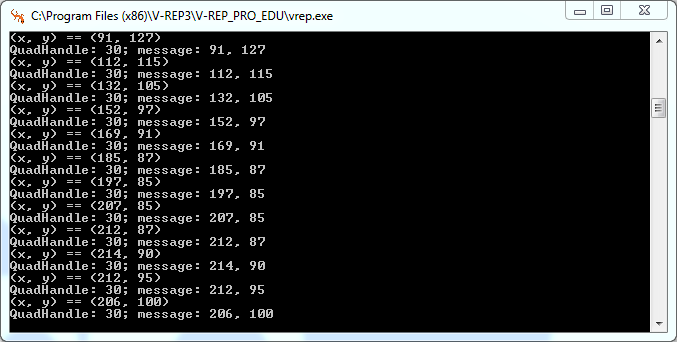
\includegraphics[width=0.7\textwidth,natwidth=677,natheight=342]{../Images/c3/ground_tracking_vrep_console.png}
	\caption{Ground Tracking V-REP Console}
	\label{fig:Ground_Tracking_VREP_Console}
\end{figure}

There is another component in the simulations, the ground station, with the aim to make the most realistic simulations, this ground station is exactly the same as real test ground station. This is possible due to the abstraction of the communication through sockets. The ground station has a simple interface to get some information about the progress. An example of this interface is shown in the Figure: \ref{fig:Ground_Tracking_Server_Console}.

\begin{figure}[h]
	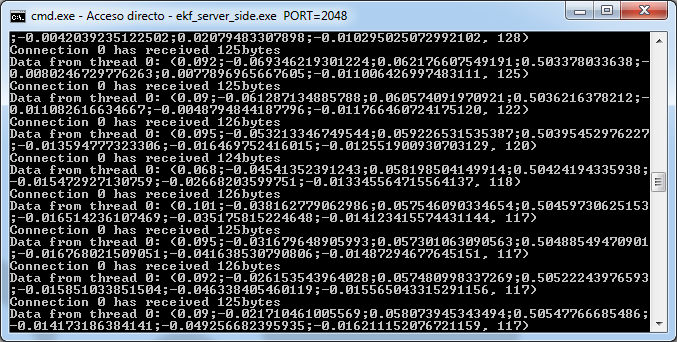
\includegraphics[width=0.7\textwidth,natwidth=677,natheight=342]{../Images/c3/ground_tracking_server_console.png}
	\caption{Ground Tracking Server Console}
	\label{fig:Ground_Tracking_Server_Console}
\end{figure}

Both ground station and objects in the simulation generate a LOG in order to analyze afterwards the results.

%-------------------------------------------------------------------------------------------------------
%-------------------------------------------------------------------------------------------------------
%-------------------------------------------------------------------------------------------------------
\subsection{Simulation 1 - Simple ground camera tracking. Vertical camera}
\subsubsection{Set up}
This Scene has basically one quad rotor and one target (Figure: \ref{fig:VREP_scene_example}). The Red sphere is moving on the floor (Describing a circle) while the quad's camera capture pictures and the on board (simulated) computer process it and command the drone in order to follow the target. In this simulation the camera is facing the ground (Figure: \ref{fig:ground_tracking_scene_vertical}).

\begin{figure}[h]
	\centering
	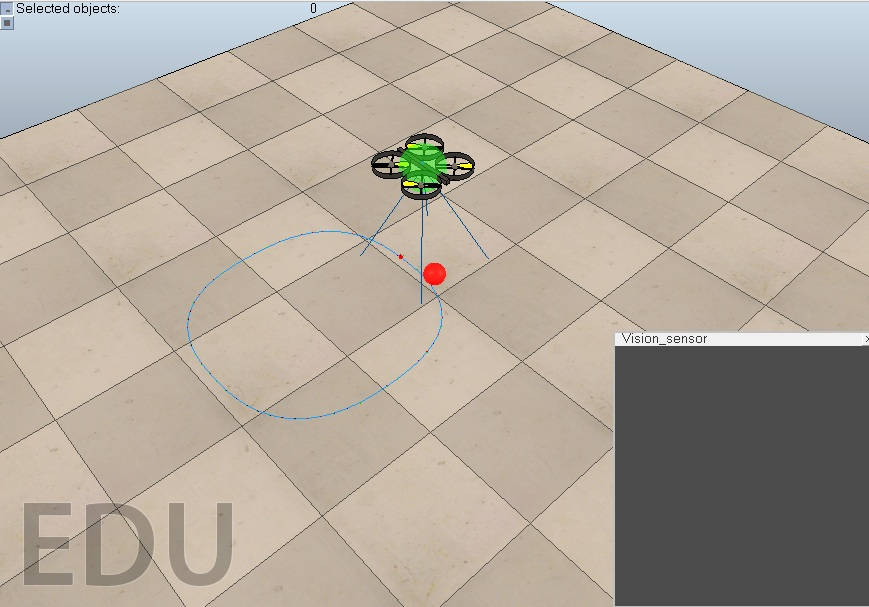
\includegraphics[width=0.7\linewidth]{../Images/c3/ground_tracking_scene_vertical}
	\caption{Ground tracking - Oblique Camera}
	\label{fig:ground_tracking_scene_vertical}
\end{figure}

\subsubsection{Test and results}


\begin{figure}[h]
	\centering
	\begin{subfigure}[b]{0.4\linewidth}
		\centering
		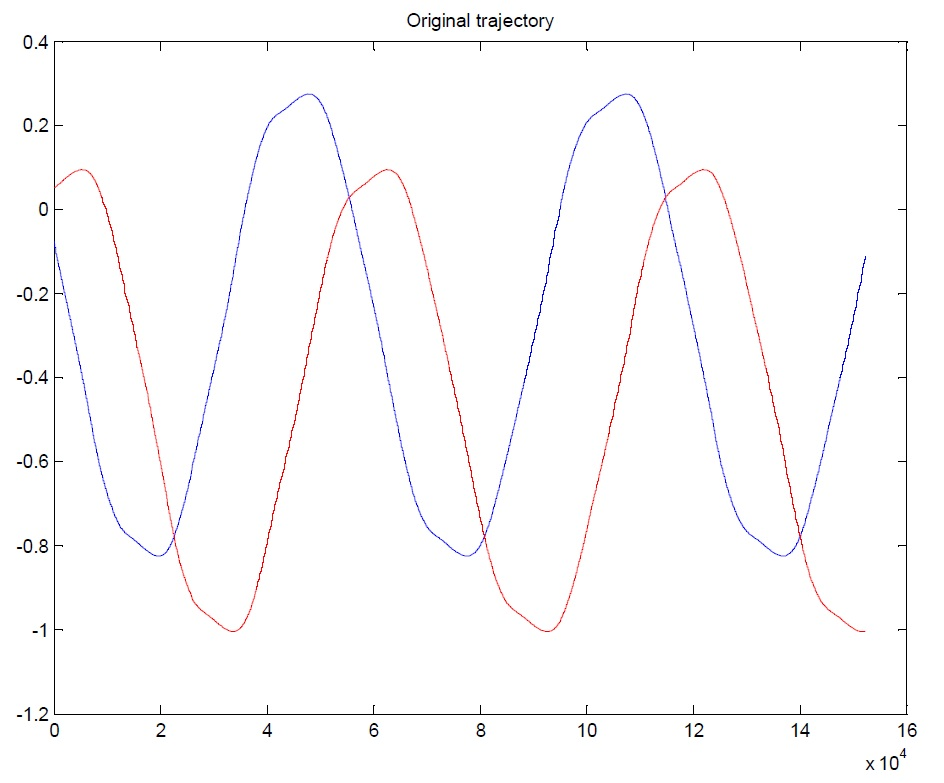
\includegraphics[width=\linewidth]{../Images/c3/sim1_traj_ori}
		\caption{Ground tracking - Original trajectory}
		\label{fig:sim1_traj_ori}
	\end{subfigure}
	~
	\begin{subfigure}[b]{0.4\linewidth}
		\centering
		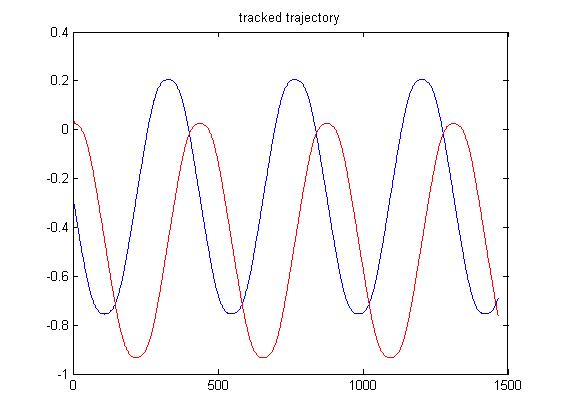
\includegraphics[width=\linewidth]{../Images/c3/sim1_traj_track}
		\caption{Ground tracking - Tracked trajectory}
		\label{fig:sim1_traj_track}
	\end{subfigure}

\end{figure}


\begin{figure}[h]
\centering
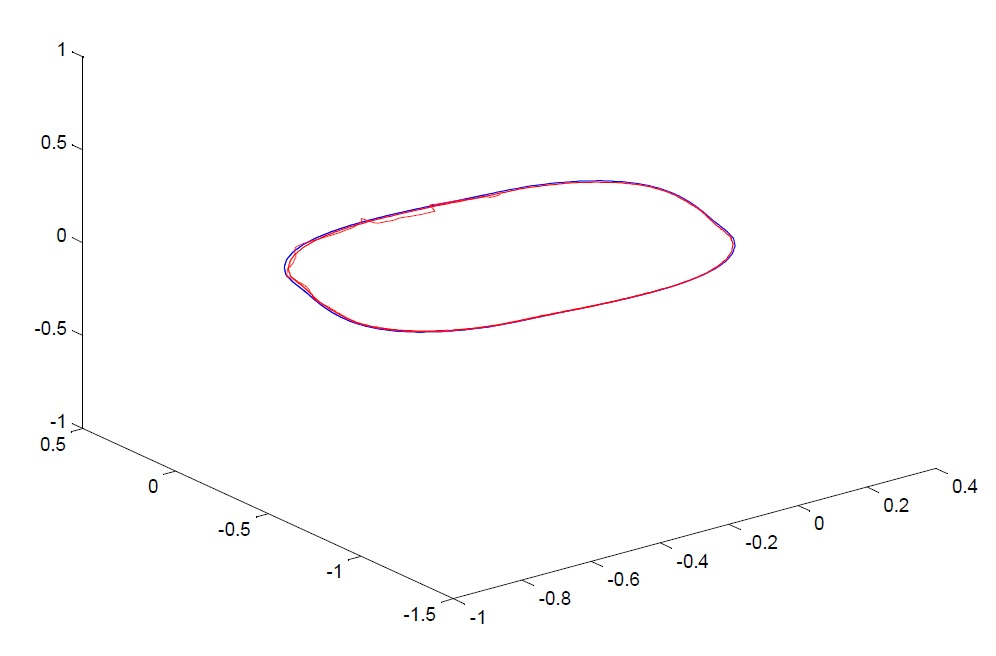
\includegraphics[width=0.7\linewidth]{../Images/c3/sim1_traj_both_3d}
\caption{Ground tracking - Oblique Camera - 3D trajectory}
\label{fig:sim1_traj_both_3d}
\end{figure}




%-------------------------------------------------------------------------------------------------------
%-------------------------------------------------------------------------------------------------------
%-------------------------------------------------------------------------------------------------------
\subsection{Simulation 2 - Simple ground camera tracking. Oblique camera}
\subsubsection{Set up}
This Scene has basically one quad rotor and one target. The Red sphere is moving on the floor (Describing a curve) while the quad's camera capture pictures and the on board (simulated) computer process it and command the drone in order to follow the target. In this case, the camera is not facing directly the ground, now it's oblique (45 degrees from the previous; Figure: \ref{fig:ground_tracking_scene_oblique}).

\begin{figure}[h]
	\centering
	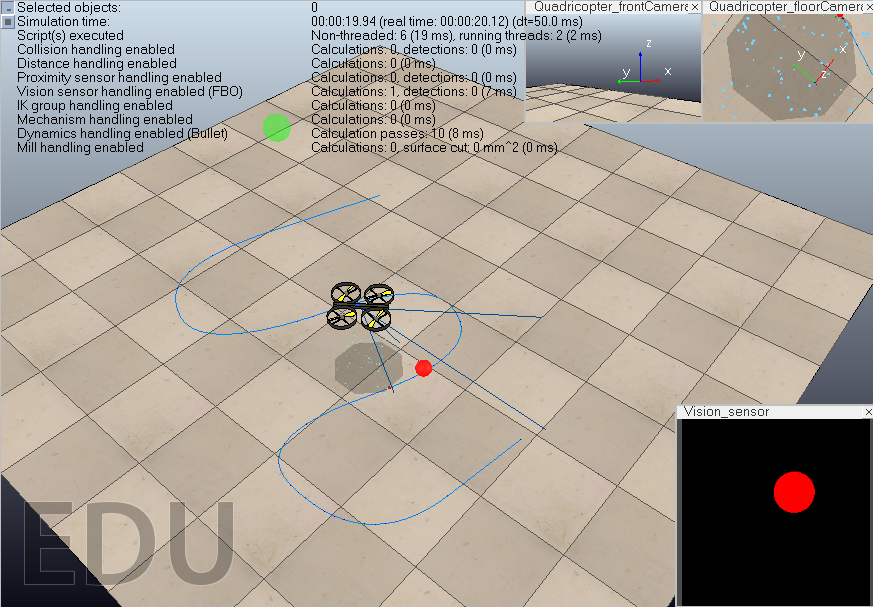
\includegraphics[width=0.7\linewidth]{../Images/c3/ground_tracking_scene_oblique}
	\caption{Ground tracking - Oblique Camera}
	\label{fig:ground_tracking_scene_oblique}
\end{figure}

\subsubsection{Test and results}


\begin{figure}[h]
	\centering
	\begin{subfigure}[b]{0.4\linewidth}
		\centering
		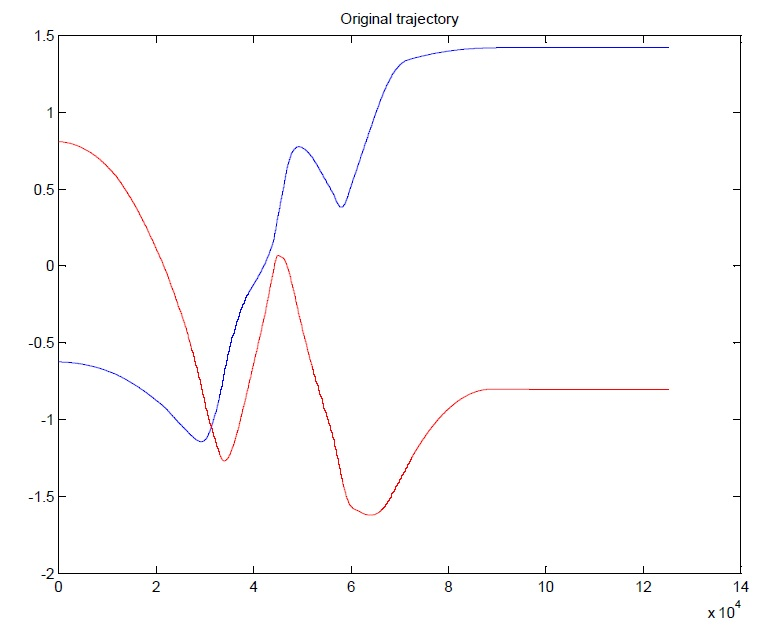
\includegraphics[width=\linewidth]{../Images/c3/sim2_traj_ori}
		\caption{Ground tracking - Original trajectory}
		\label{fig:sim2_traj_ori}
	\end{subfigure}
	~
	\begin{subfigure}[b]{0.4\linewidth}
		\centering
		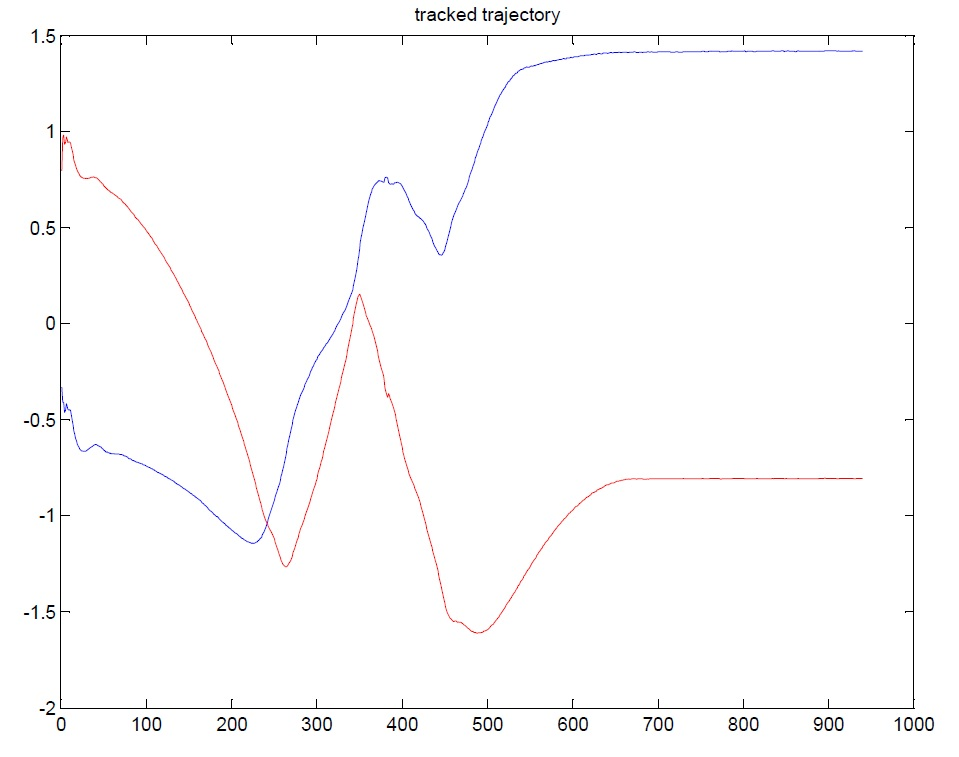
\includegraphics[width=\linewidth]{../Images/c3/sim2_traj_track}
		\caption{Ground tracking - Tracked trajectory}
		\label{fig:sim2_traj_track}
	\end{subfigure}

\end{figure}


\begin{figure}[h]
\centering
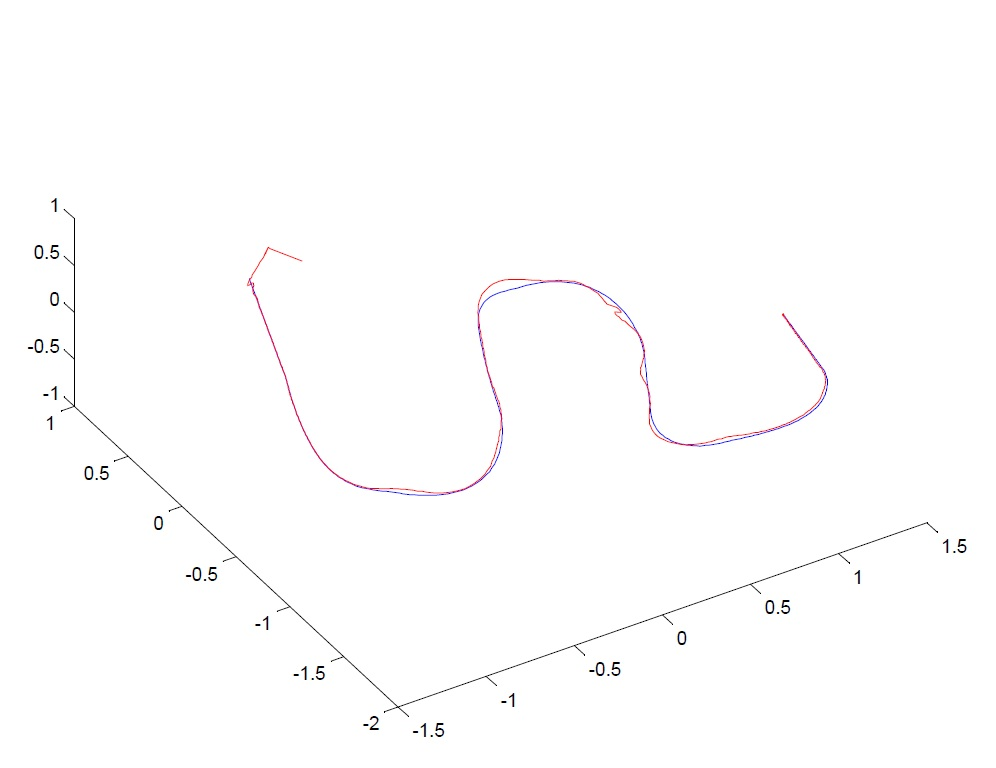
\includegraphics[width=0.7\linewidth]{../Images/c3/sim2_traj_both_3d}
\caption{Ground tracking - Oblique Camera - 3D trajectory}
\label{fig:sim2_traj_both_3d}
\end{figure}




%-------------------------------------------------------------------------------------------------------
%-------------------------------------------------------------------------------------------------------
%-------------------------------------------------------------------------------------------------------
\subsection{Stereo tracking}
\subsubsection{Set up}
\subsubsection{Test and results}